\documentclass{standalone}
\usepackage{tikz}
\usepackage{amsmath, amssymb}

\begin{document}

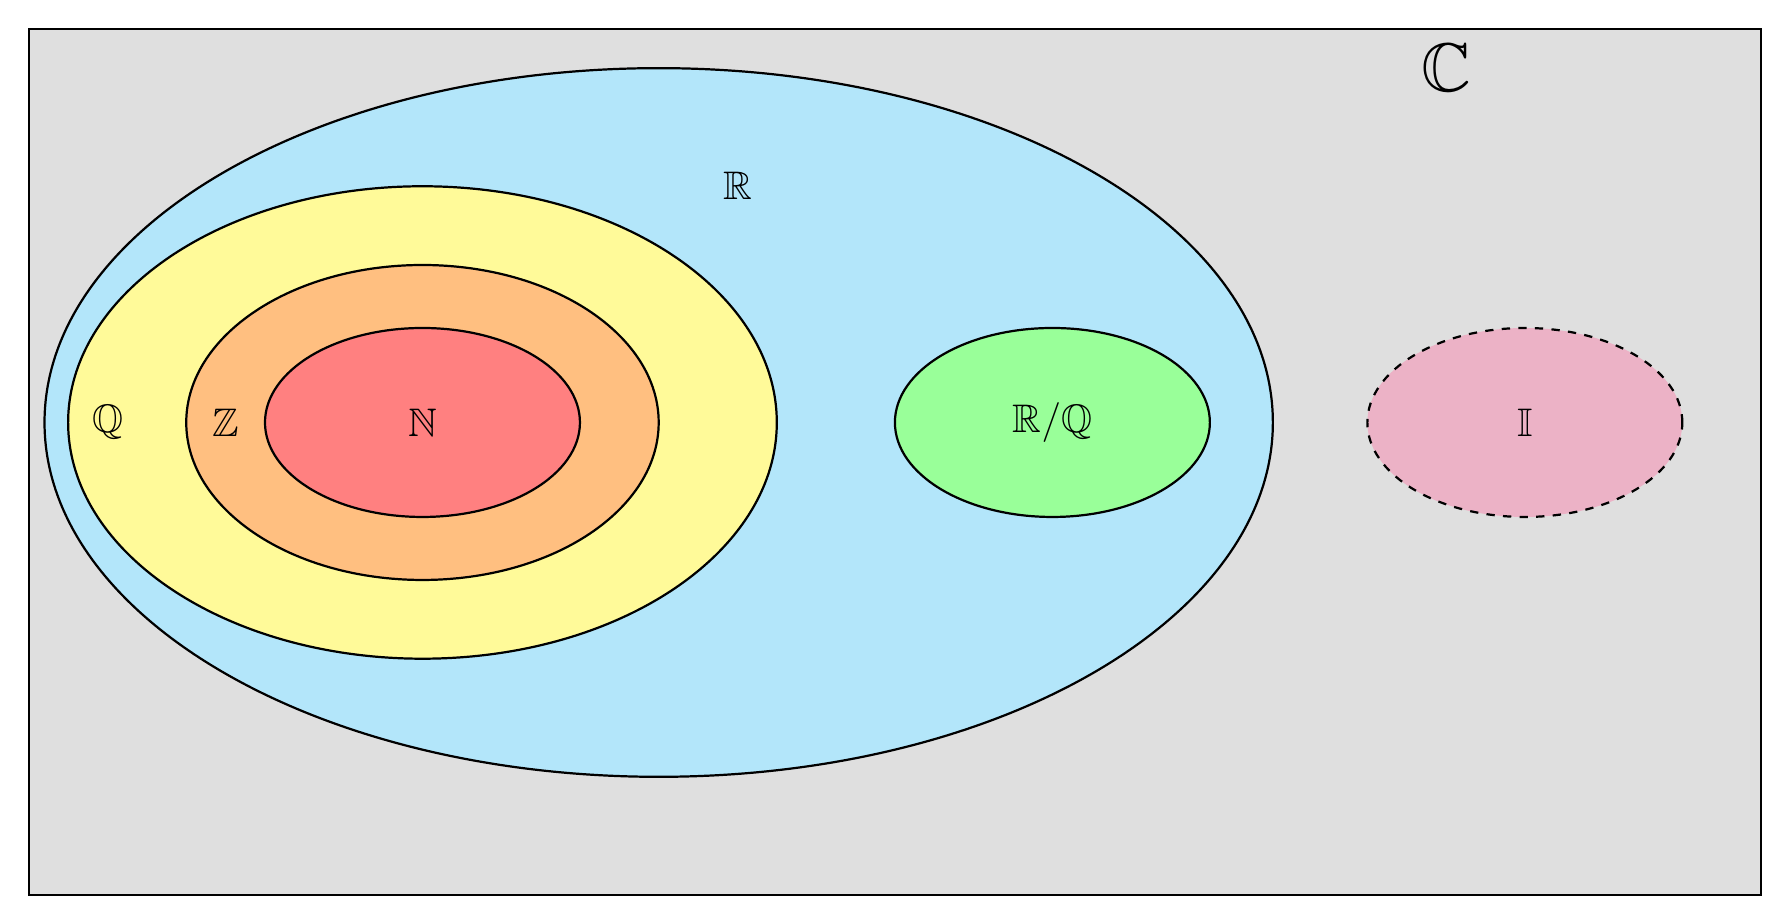
\begin{tikzpicture}

    % Complex Numbers (outer square)
    \draw[thick, fill=lightgray!50] (-12, -6) rectangle (10, 5);
    \node at (6, 4.5) {\Huge $\mathbb{C}$};
    
    % Real Numbers (largest set)
    \draw[thick, fill=cyan!30] (-4,0) ellipse (7.8cm and 4.5cm);
    \node at (-3, 3) {\Large $\mathbb{R}$};
    
    % Rational Numbers
    \draw[thick, fill=yellow!40] (-7,0) ellipse (4.5cm and 3cm);
    \node at (-11, 0) {\Large$\mathbb{Q}$};
    
    % Integers
    \draw[thick, fill=orange!50] (-7,0) ellipse (3cm and 2cm);
    \node at (-9.5, 0) {\Large$\mathbb{Z}$};
    
    % Natural Numbers
    \draw[thick, fill=red!50] (-7,0) ellipse (2cm and 1.2cm);
    \node at (-7, 0) {\Large$\mathbb{N}$};
    
    % Irrational Numbers
    \draw[thick, fill=green!40] (1,0) ellipse (2cm and 1.2cm);
    \node at (1, 0) {\Large$\mathbb{R} /\mathbb{Q} $};
    
    % Imaginary Numbers
    \draw[thick, dashed, fill=purple!30] (7,0) ellipse (2cm and 1.2cm);
    \node at (7, 0) {\Large $\mathbb{I}$};

\end{tikzpicture}

\end{document}
